\documentclass{beamer}

%Information to be included in the title page:
\title{Risk Management}

\author{Charles Rambo}

\date{5/9/2022}


\AtBeginSection[]{
  \begin{frame}
  \vfill
  \centering
  \begin{beamercolorbox}[sep=8pt,center,shadow=true,rounded=true]{title}
    \usebeamerfont{title}\insertsectionhead\par%
  \end{beamercolorbox}
  \vfill
  \end{frame}
}


\usepackage{tikz}
\usepackage{pgfplots}
\usepackage{bm}
\usepackage{amsthm}
\usepackage{graphicx}

\addtobeamertemplate{navigation symbols}{}{%
    \usebeamerfont{footline}%
    \usebeamercolor[fg]{footline}%
    \hspace{1em}%
    \insertframenumber/\inserttotalframenumber
}

\newtheorem*{remark}{Remark}

\setbeamertemplate{section in toc}[sections numbered]
\setbeamertemplate{subsection in toc}[subsections numbered]

\begin{document}

\frame{\titlepage}

\begin{frame}
\frametitle{Table of Contents}
\tableofcontents
\end{frame}

\section{Objective}

\begin{frame}
\frametitle{Objective}
\begin{itemize}
\item Introduce the concepts necessary to understand portfolio risk metrics.
\item Provide some risk management metrics to help access risk within Outright portfolios. 
\item Work with Client Services to integrate some formulation of the metrics into regular reports to current and prospective clients.
\end{itemize}
\end{frame}


\section{Key Concepts}

\subsection{What Is VaR?}

\begin{frame}
\frametitle{What Is VaR?}
The value-at-risk (VaR) of a portfolio is the largest  ``reasonable" loss that could occur. For a significance level $\alpha$, the $(100\% - \alpha)$-VaR measures the distance between neutral and the $\alpha$-th percentile.
\bigskip

\begin{center}

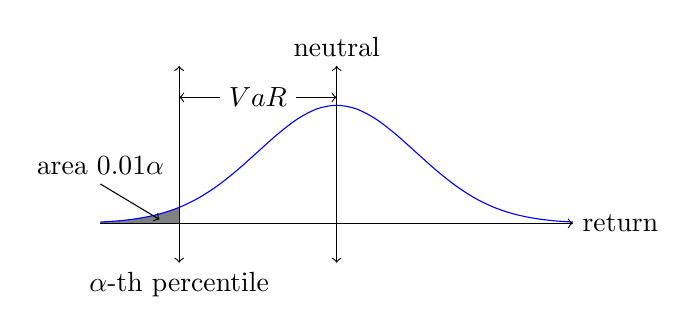
\begin{tikzpicture}

\fill[gray, domain=-3:-2, variable=\x] (-3, 0) -- plot ({\x}, {1.5 * exp(-0.5 * \x * \x)}) -- (-2, 0) -- cycle;

\draw[domain = -3:3, smooth, variable =\x,  blue] plot ({\x}, {1.5 * exp(-0.5 * \x * \x)});

\draw[<->] (0, -0.5) -- (0, 2)  node[above] {neutral};
\draw[<->] (-2, 2) -- (-2, -0.5) node[below]{$\alpha$-th percentile};

\draw[->] (-3, 0) -- (3, 0) node[right]{return};

\draw[<-] (-2.25, 0.05) -- (-3, 0.5) node[above] {area $0.01\alpha$};

\draw[<->] (-2, 1.6) -- (0, 1.6);

\node[fill = white] at (-1, 1.6) {$VaR$};

\end{tikzpicture}

\end{center}

\end{frame}

\begin{frame}
\frametitle{What Is VaR?}

\begin{itemize}
\item  The \textbf{significance level} is $\alpha$.
\item The \textbf{confidence level} is $100\% - \alpha$. This is how certain we are that we won't experience a loss greater than the VaR.
\item The $\boldsymbol{(100\% - \alpha)}$\textbf{-VaR} is neutral minus the $\alpha$-th percentile. Typically, in risk management we consider 0 to be the ``neutral"  return.
\item An \textbf{exception} occurs when the loss exceeds the VaR.  A good VaR estimate should have an average of about $\alpha$ exceptions.
\end{itemize}

\end{frame}

\begin{frame}
\frametitle{What Is VaR?}
\begin{example}
Suppose the daily return $R$ of a portfolio follows a normal distribution with mean 0 and variance $0.013^2$, i.e. 
$$R\sim{\mathcal{N}(0,0.013^2)}.$$ 
What is the 95\%-VaR?
\end{example}
\end{frame}

\begin{frame}
\frametitle{What Is VaR?}

\begin{center}

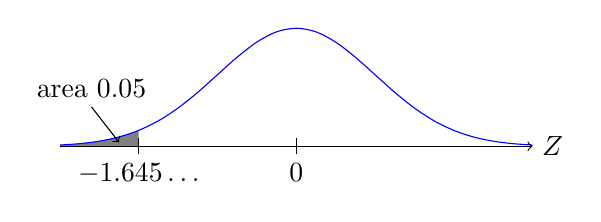
\begin{tikzpicture}

\fill[gray, domain=-3:-2, variable=\x] (-3, 0) -- plot ({\x}, {1.5 * exp(-0.5 * \x * \x)}) -- (-2, 0) -- cycle;

\draw[domain = -3:3, smooth, variable =\x,  blue] plot ({\x}, {1.5 * exp(-0.5 * \x * \x)});


\draw (-2, 0.1) -- (-2, -0.1) node[below]{$-1.645\ldots$};

\draw (0, 0.1) -- (0, -0.1) node[below]{0};

\draw[->] (-3, 0) -- (3, 0) node[right]{$Z$};

\draw[<-] (-2.25, 0.05) -- (-2.6, 0.5) node[above] {area 0.05};



\end{tikzpicture}

\end{center}

\begin{solution}
We can use a standard normal table to answer this question.  Five percent of the area under the standard normal distribution is to the left of  $Z\approx-1.645$. Hence, if fifth return percentile is $R_5$,
$$
\frac{R_5 - 0}{0.013} \approx -1.645\quad\text{implies}\quad R_5 \approx (-1.645)(0.013) \approx -0.0214.
$$
It follows that the value-at-risk is about
$$
0 - ( -0.0214) = 0.0214\;\text{or}\; 2.14\%.
$$
\end{solution}

\end{frame}

\begin{frame}
\frametitle{What Is VaR?}
\begin{remark}
The normal distribution is often a poor choice for modeling the tail behavior of returns. The normal distribution's tails are very thin!
\includegraphics[scale = 0.4]{norm_tail.png}
\end{remark}
\end{frame}

\begin{frame}
\frametitle{What Is VaR?}
\begin{center}
\begin{tabular}{| c | c c c |}
\hline
Event		&	Default	&	Perform Badly	&	Perform Well		\\\hline
Return	&	-100\%	&	-1\%			&	20\%			\\
Probability	&	4\%		&	26\%			&	70\%			\\\hline
\end{tabular}
\end{center}
\begin{example}
An investor's portfolio only contains the asset whose return profile is shown in the table. Compute her 95\%-VaR.
\end{example}

\end{frame}

\begin{frame}
\frametitle{What Is VaR?}
\begin{center}
\begin{tabular}{| c | c c c |}
\hline
Event		&	Default	&	Perform Badly	&	Perform Well		\\\hline
Return	&	-100\%	&	-1\%			&	20\%			\\
Probability	&	4\%		&	26\%			&	70\%			\\\hline
\end{tabular}
\end{center}
\begin{solution}
The fifth percentile of returns is -1\%. Hence, her 95\%-VaR is
$$
0 - (-1\%) = 1\%.
$$
\end{solution}

\end{frame}

\begin{frame}
\frametitle{What Is VaR?}

\begin{remark}
The value-at-risk didn't reflect the default probability of the investor's asset, because it was outside of the confidence level. 

Scenarios like this illustrate a weakness of value-at-risk. For some investments, like a small portfolio of either low credit convertible bonds, written out-of-the-money options, or non-insured mortgage-backed securities, the value-at-risk can be deceptive because it doesn't reflect extreme events outside of the confidence level.
\end{remark}

\begin{center}

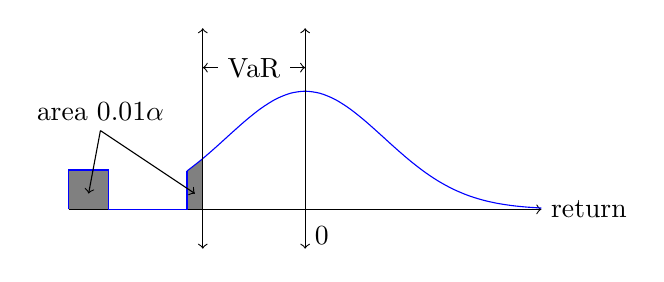
\begin{tikzpicture}

\fill[gray] (-3, 0) -- (-3, 0.5) -- (-2.5, 0.5) -- (-2.5, 0) -- cycle;

\fill[gray, domain=-1.5:-1.3, variable=\x] (-1.5, 0) -- plot ({\x}, {1.5 * exp(-0.5 * \x * \x)}) -- (-1.3, 0) -- cycle;

\draw[->] (-3, 0) -- (3, 0) node[right]{\text{return}};

\draw[domain = -1.5:3, smooth, variable =\x,  blue] plot ({\x}, {1.5 * exp(-0.5 * \x * \x)});

\draw[blue] (-3, 0) -- (-3, 0.5) -- (-2.5, 0.5) -- (-2.5, 0) -- (-1.5, 0) -- (-1.5, 0.487);

\draw[<-] (-2.75, 0.2) -- (-2.6, 1) node[above] {area $0.01\alpha$};
\draw[<-] (-1.4, 0.2) -- (-2.6, 1);

\draw (0, 0.1) -- (0, -0.1) node[below right]{0};

\draw[<->] (-1.3, 2.3) -- (-1.3, -0.5);

\draw[<->] (0, 2.3) -- (0, -0.5);

\draw[<->] (-1.3, 1.8) -- (0, 1.8);

\node[fill = white] at (-0.65, 1.8) {VaR};

\end{tikzpicture}

\end{center}

\end{frame}

\subsection{What Is Expected Shortfall?}

\begin{frame}
\frametitle{What Is Expected Shortfall?}
The $\boldsymbol{100\% - \alpha}$ \textbf{expected shortfall} of a portfolio's return is the expected value of the return given that the loss is less than or equal to the $(100\% - \alpha)$-VaR. 
\bigskip

That is, if the $(100\% - \alpha)$-VaR is $v$ and  $R$ is the random variable representing returns, the $100\% - \alpha$ expected shortfall is
$$
E\Big[R\Big| R \leq -v\Big].
$$
\end{frame}

\begin{frame}
\frametitle{What Is Expected Shortfall?}
\begin{center}
\begin{tabular}{| c | c c c |}
\hline
Event		&	Default	&	Perform Badly	&	Perform Well		\\\hline
Return	&	-100\%	&	-1\%			&	20\%			\\
Probability	&	4\%		&	26\%			&	70\%			\\\hline
\end{tabular}
\end{center}
\begin{example}
An investor's portfolio only contains the asset whose return profile is shown in the table. Compute her 95\% expected shortfall.
\end{example}
\end{frame}


\begin{frame}
\frametitle{What Is Expected Shortfall?}
\begin{center}
\begin{tabular}{| c | c c c |}
\hline
Event		&	Default	&	Perform Badly	&	Perform Well		\\\hline
Return	&	-100\%	&	-1\%			&	20\%			\\
Probability	&	4\%		&	26\%			&	70\%			\\\hline
\end{tabular}
\end{center}
\begin{solution}
Given that we are below the fifth percentile, the probability of default is $4/5 = 80\%$ and the probability of poor performance is $1 - 4/5 = 20\%$. There is no chance the asset performs well. Hence, her expected shortfall is
$$
0.80(-100\%) + 0.20(-1\%) = -80.2\%.
$$
\end{solution}

\end{frame}


\begin{frame}
\frametitle{What Is Expected Shortfall?}
\begin{example}
The return $R$ of a portfolio follows a Gau{\ss}ian mixture model with states 1 and 2. In state 1, the expected return is $-0.2\%$  and the variance $0.40^2/250$. In state 2, the expected  return is $0.1\%$ and the variance is $0.20^2/250$. The probability of states 1 and 2 are 25\% and 75\%, respectively. In other words,
$$
R\sim{0.25\mathcal{N}\left(-0.002, \frac{0.40^2}{250}\right) + 0.75\mathcal{N}\left(0.001, \frac{0.20^2}{250}\right)}. 
$$
What are the 95\% value-at-risk and expected shortfall?
\end{example}
\end{frame}

\begin{frame}
\frametitle{What Is Expected Shortfall?}
\begin{solution}
Let's use a Monte Carlo simulation. We will sample 100,000 values from the mixture model. Then we will calculate the VaR and expected shortfall using the simulated data.
\begin{center}
\includegraphics[scale = 0.4]{mix_norm.png}
\end{center}
The fifth percentile from our sample is $-2.74\%$. It follows that the value-at-risk is about 2.74\%. The expected shortfall is the mean return excluding returns above -2.74\%. This value is about -3.92\%. So, the expected shortfall is -3.92\%.
\end{solution}
\end{frame}

\subsection{What Is a GARCH Model?}

\begin{frame}
\frametitle{What Is a GARCH Model?}
The volatility of returns changes over time. The graph of S\&P 500 returns shows that at times returns oscillate within a narrow range while at other times returns exhibit wild swings. Such behavior would be almost impossible under the assumption of constant volatility. 
\begin{center}
\includegraphics[scale = 0.4]{spx.png}
\end{center}

\end{frame}

\begin{frame}
\frametitle{What Is a GARCH Model?}
To model financial market volatility, a common assumption is that it follows a GARCH(1,1) model. That is, it is common to assume that the time $t$ volatility $\sigma_t$ is governed by the equation
$$
\sigma_t^2 = \omega + \alpha\epsilon_{t - 1}^2 + \beta\sigma_{t-1}^2,
$$
where $\alpha, \beta, \omega \geq 0$, and the return $ r_t \sim{\mathcal{N}(\mu, \sigma_t^2)}$.
\end{frame}

\begin{frame}

\frametitle{What Is a GARCH Model?}
\begin{example}
Suppose each S\&P 500 return $r_t\sim{\mathcal{N}(0, \sigma_t^2)}$, where $\sigma_t$ is governed by a GARCH(1, 1) model. Plot the negative 95\%-VaR over time on the S\&P 500 time series return graph. Show value-at-risk exceptions.
\end{example}

\begin{solution}
\includegraphics[scale = 0.4]{spx_var.png}
\end{solution}

\end{frame}

\begin{frame}
\frametitle{What Is a GARCH Model?}
\begin{remark}
This value-at-risk model isn't great! All of the exceptions are bunched up during the start of the Covid crisis. A good model should have no bunching. Exceptions are supposed to be unpredictable. Furthermore, exceptions occur less than 5\% of the time.
\end{remark}

\end{frame}

\section{Results}

\subsection{Time Series Method}

\begin{frame}
\frametitle{Time Series Method}

Use time series data, a GARCH(1,1) model, and the lognormal distribution to estimate the left tail of returns. Then use the estimate to calculate VaR and expected shortfall.
\begin{itemize}
\item Fit the time $t$ parameters of the GARCH(1,1) model using returns from $t-75$ to $t-1$. Use the results to predict the time $t$ volatility.
\item Standardize time $t$ returns by dividing by its predicted volatility. Fit a lognormal distribution to the bottom 40\% of time $t-75$ to $t-1$ standardized returns.
\item Model the VaR and expected shortfall with the estimated values.
\end{itemize}

\end{frame}

\begin{frame}

\frametitle{GARCH(1, 1)}
Use the returns $r_{t-1}, r_{t-2},\ldots, r_{t-75}$ to estimate the parameters of a GARCH(1,1) model. Then use the GARCH(1, 1) model to predict the time $t$ volatility.
\begin{center}
\includegraphics[scale = 0.25]{garch.png}
\end{center}

\end{frame}

\begin{frame}
\frametitle{Standardize Returns and Estimate the Left Tail}

For each time $t$, standardize the return $r_t$ by dividing by its predicted volatility $\sigma_t$, i.e. calculate $\tilde{r_t} =  r_t/\sigma_t$. Fit a lognormal distribution to the bottom 40\% of standardized returns $\tilde{r_t}$. 
\begin{center}
\includegraphics[scale = 0.25]{lognorm.png}
\end{center}

\end{frame}

\begin{frame}
\frametitle{VaR and Expected Shortfall}
\begin{center}
\includegraphics[scale = 0.25]{ts_port.png}

\begin{tabular}{| c | c c c |}
\hline
Account	&	95\%-VaR	&	VaR Exceptions	&	Expected Shortfall\\\hline
Citi        	&	1.99\% 		&       4.23\%			&              -2.38\%\\
VXA0        	&	1.63\%		&       5.00\%			&               -2.19\%\\
Chesapeake  &	1.43\%		&        5.00\%			&               -2.01\%\\
V0S1        	&	1.70\%		&        5.00\%			&              -2.58\%\\
\hline
\end{tabular}

\end{center}

\end{frame}


\begin{frame}
\frametitle{Data}

Daily time series return data from 1/1/2021 to 4/30/2022. Accessed on Clearwater 5/5/2022.

\end{frame}


\begin{frame}
\frametitle{Pros and Cons}

{\bf Pros}\hspace{0.5\textwidth}{\bf Cons}

\begin{columns}
\column{.5\textwidth}
\begin{itemize}
\item Easy to backtest. 
\item ``Straightforward" construction.
\item Easy to visualize change in risk over time.
\end{itemize}
\column{.5\textwidth}
\begin{itemize}
\item Parameter calibration can be sensitive. Sometimes results may seem a bit ``off".
\item The model has few applications other than VaR and expected shortfall calculations. 
\item Doesn't help find the primary drivers of the risk within a portfolio.
\end{itemize}
\end{columns}

\end{frame}


\subsection{Monte Carlo Method}

\begin{frame}
\frametitle{Monte Carlo Method}
Simulates portfolio returns based on underlying equity and interest rate fluctuations. Then use the simulation to calculate VaR and expected shortfall.
\begin{itemize}
\item Use a mixture model to simulate market returns.
\item Model equity returns using the CAPM framework. 
\item Use a scaled Student's $t$-distribution to model changes in interest rates.
\item Estimate the change in each security's price using $\Delta$, $\Gamma$, duration $D$, and interest rate convexity $C$. 
\item Simulate default using Bloomberg probabilities and the uniform distribution $\mathcal{U}[0, 1]$. 
\item Use the portfolio weights and the simulated security level returns to obtain portfolio level returns.
\item Model the VaR and expected shortfall with the simulated portfolio level returns.
\end{itemize}
\end{frame}

\begin{frame}
\frametitle{Market Returns}
The model assumes that market returns $r_{mkt}$ follow a mixture model with states $bad$ and $good$. That is, we suppose
$$
r_{mkt}\sim{\pi_{bad}\mathcal{N}(\mu_{bad}, \sigma_{bad}^2) + \pi_{good}\mathcal{N}(\mu_{good}, \sigma_{good}^2)}.
$$
The state $bad$ represents bad times in the market and the state $good$ represents good times. As a result, we expect
$$
\mu_{bad} < \mu_{good}\quad\text{and}\quad \sigma_{bad} > \sigma_{good}.
$$
\end{frame}

\begin{frame}
\frametitle{Equity Returns}
The CAPM framework claims the equity return corresponding to security $i$ is governed by the equation
$$
r_i^{equity} = r_{riskfree} + \beta_i (r_{mkt} - r_{riskfree}) + \epsilon_i,
$$
where $\epsilon_i\sim{\mathcal{N}(0, \sigma_i^2)}$.

It follows that
$$
Var(r_i^{equity}) = \beta_i^2 Var(r_{mkt}) + \sigma_i^2.
$$
There are several equity return volatility metrics available. Any one of them allows us to solve for $\sigma_i$.

During bad times $\beta_i$ tends to increase. So, we break $\beta_i$ into two cases. We assume
$$
\beta_i^{bad} = 1.30\beta_i\quad\text{and}\quad \beta_i^{good} = \frac{1  - 1.30\pi_{bad}}{\pi_{good}}\beta_i.
$$
\end{frame}

\begin{frame}
\frametitle{Interest Rates}
For security $i$ with tenor $T$, we model the fluctuation in the bond's discount rate by
$$
r_i^{fixed} = (r_{US, T} + s_i)(1 + X),
$$
where $r_{US, T}$ is the discount rate of a US treasury bond of tenor $T$ and $s_i$ is the spread of security $i$. We suppose $X$ follows a scaled Student's $t$-distribution.
\end{frame}


\begin{frame}
\frametitle{Security Price}
Let's say the security price $B_i = f(S_i, r_i)$, where $S_i$ denotes the equity price of security $i$ and $r_i$ its discount rate. Then, after making a few assumptions about $f$, Taylor's theorem tells us
\begin{align*}
B_i^{new} - B_i^{old} &\approx \frac{\partial B_i}{\partial S_i} (S_i^{new} - S_i^{old}) + \frac{\partial B_i}{\partial r_i}(r_i^{new} - r_i^{old})\\
				&\qquad + \frac{1}{2}\frac{\partial^2 B_i}{\partial S_i^2} (S_i^{new} - S_i^{old})^2\\ 
				&\qquad + \frac{\partial^2 B_i}{\partial S_i\partial r_i}(S_i^{new} - S_i^{old}) (r_i^{new} - r_i^{old})\\
				&\qquad + \frac{1}{2}\frac{\partial^2 B_i}{\partial r_i^2}(r_i^{new} - r_i^{old})^2.
\end{align*}


\end{frame}

\begin{frame}
\frametitle{Security Price Continued}
Many of these values are known:
$$
\Delta = \frac{\partial B}{\partial S},\quad \frac{\partial B}{\partial r} = -B\cdot D,\quad \Gamma = \frac{\partial^2 B}{\partial S^2},\quad\text{and}\quad \frac{\partial^2 B}{\partial r^2} = B \cdot C.
$$
We assume the partial derivative 
$$
\frac{\partial^2 B}{\partial S\partial r} = 0.\footnotemark
$$
Since 
$$
S^{new} - S^{old} = S^{old}\cdot r^{equity}\quad\text{and}\quad r^{new} - r^{old} = r^{old}\cdot X,
$$
it follows that
\begin{align*}
B_i^{new} - B_i^{old} 	&\approx \Delta_i\cdot S_i^{old}\cdot r_i^{equity}  - B_i\cdot D_i\cdot r_i^{old}\cdot X \\
				&\qquad + \frac{1}{2}\cdot \Gamma_i\cdot  (S_i^{old}\cdot r_i^{equity})^2  + \frac{1}{2}\cdot B_i\cdot D_i\cdot (r_i^{old}\cdot X)^2.
\end{align*}

\footnotetext[1]{For a regular convertible bond using the Black-Scholes framework, 
$$
\frac{\partial^2 B}{\partial S\partial r} = \phi(d_1)\cdot \frac{\sqrt{T}}{\sigma}.
$$
}
\end{frame}

\begin{frame}
\frametitle{Default}
Suppose $p_i$ is the one-year probability of default. We first convert $p_i$ to a daily probability via
$$
p_i^{daily} = 1 - (1 - p_i)^{1/250}.
$$
Furthermore, we assume all defaults occur in the $bad$ market state. The probability of default in this state is
$$
q_i = \frac{p_i^{daily}}{\pi_{bad}}.
$$
Draw a $U_i$ from the uniform distribution $\mathcal{U}[0, 1]$. If $U_i < q_i$, we suppose the firm defaults and the recovery rate is \$25 per \$100 of par.
\end{frame}

\begin{frame}
\frametitle{VaR and Expected Shortfall (Ex Cash)}
\begin{center}
\includegraphics[scale = 0.25]{monte_carlo_port.png}

\begin{tabular}{| c | c c |}
\hline
Account	&	95\%-VaR	&	Expected Shortfall\\\hline
Citi		&	2.27\%	&          -3.95\% \\
VXA0		&	2.30\%	&          -3.83\%	\\
Chesapeake	&	1.46\%	&          -2.47\%	\\
V0S1		&	1.35\%	&          -2.24\%\\\hline
\end{tabular}

\end{center}

\end{frame}

\begin{frame}
\frametitle{Data}
\begin{itemize}
\item Mixture model fit on S\&P 500 data from 1/1/2020 to 4/30/2022.
\item Scaled Student's $t$-distribution fit on percent changes in five-year treasury yield data. Data from 1/1/2020 to 4/30/2022.
\item Portfolio weights as of 4/30/22.
\item Bloomberg security level metrics pulled on 4/29/2022.
\end{itemize}


\end{frame}


\begin{frame}
\frametitle{Pros and Cons}

{\bf Pros}\hspace{0.5\textwidth}{\bf Cons}

\begin{columns}
\column{.5\textwidth}
\begin{itemize}
\item Easy to do scenario analysis.
\begin{enumerate}
\item[-] What happens if the S\&P 500 drops 5\%?
\item[-] How much will the risk profile improve if duration is reduced by 10\%?
\item[-] How would the risk profile change if we removed securities X and Y?
\end{enumerate}
\item Construction consistent with how portfolios are currently being analyzed.
\begin{enumerate}
\item[-] Looks at $\Delta$'s, $\beta$'s, interest rate durations and convexities, etc.
\end{enumerate}
\end{itemize}
\column{.5\textwidth}
\begin{itemize}
\item Difficult to backtest.
\item Probably less accurate. 
\item May be difficult to understand. 
\end{itemize}
\end{columns}

\end{frame}


\begin{frame}

\end{frame}
\end{document}